\documentclass[11pt, oneside]{article}   	% use "amsart" instead of "article" for AMSLaTeX format
\usepackage[margin=1in]{geometry}                		% See geometry.pdf to learn the layout options. There are lots.
\geometry{letterpaper}                   		% ... or a4paper or a5paper or ... 
%\geometry{landscape}                		% Activate for rotated page geometry
%\usepackage[parfill]{parskip}    		% Activate to begin paragraphs with an empty line rather than an indent
\usepackage{graphicx}				% Use pdf, png, jpg, or eps§ with pdflatex; use eps in DVI mode
								% TeX will automatically convert eps --> pdf in pdflatex		
\usepackage{amssymb}
\usepackage{undertilde}

\usepackage[T1]{fontenc}
\usepackage{mathtools}  % loads »amsmath«
\usepackage{physics}

\setlength{\parskip}{0.5em}
%SetFonts

%SetFonts
\newcommand\Rey{\mbox{\textit{Re}}}

\title{\vspace{-6ex}\Large VISUALIZATION OF STREAMLINES FOR FLOW PAST A STOKESLET}
\author{\vspace{-6ex}Anup V Kanale}
\date{\vspace{-3ex}\today}							% Activate to display a given date or no date

\begin{document}
\maketitle
\section*{\vspace{-2ex} THEORY}
A stokeslet is the solution to a \textit{point force} embedded in Stokes flow. In a lot of the literature, spherical particles are approximated as Stokeslets. Therefore, understanding the Stokeslet is very fundamental to studying the interaction between particles at low Reynold's numbers.

For a $2D$ velocity flow field $\boldsymbol{u} = u\boldsymbol{\hat{i}} + v \boldsymbol{\hat{j}} $, define a stream function such that
	\begin{equation}
	v = -\pdv{\psi}{x} \quad  u = \pdv{\psi}{y}
	\end{equation}
Governing equations of Stokes Flow are given as,
	\begin{align}
 	\grad p - \mu \laplacian \boldsymbol{u} &= \boldsymbol{f} \\
 	\div \boldsymbol{u} &= 0
	\end{align}
Taking curl of the Momentum equations, we get
	\begin{align}
	\laplacian (\curl \boldsymbol{u}) &= \curl \grad p = 0 \\
	\therefore \nabla^4 \psi &= 0
	\end{align}
We see that the above equation is bi-harmonic. The streamlines for a Stokeslet in infinite domain, as obtained from the accompanying code, are as shown in the figure below.
	\begin{figure} [!htbp]
	\centering
	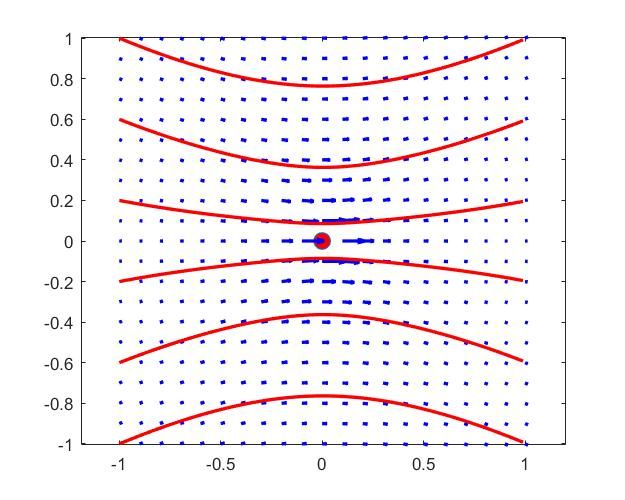
\includegraphics[scale=0.4]{StokesletStreamlines_picture}
	\caption{Flow past a Stokeslet}
	\end{figure}

\end{document}